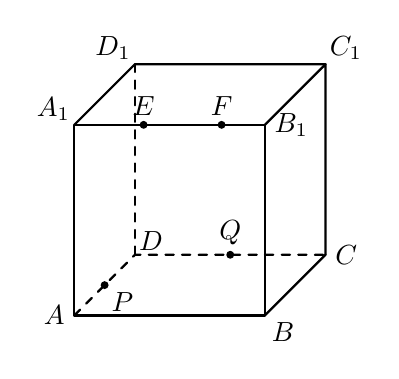
\begin{tikzpicture}[scale=1.1, line cap=round, line join=round]
  % Cube coordinates
  \coordinate (A) at (0, 0);
  \coordinate (B) at (2.2, 0);
  \coordinate (D) at (0.7, 0.7);
  \coordinate (C) at (2.9, 0.7);
  \coordinate (A1) at (0, 2.2);
  \coordinate (B1) at (2.2, 2.2);
  \coordinate (D1) at (0.7, 2.9);
  \coordinate (C1) at (2.9, 2.9);

  % Points
  \coordinate (E) at (0.8, 2.2);
  \coordinate (F) at (1.7, 2.2);
  \coordinate (P) at (0.35, 0.35);
  \coordinate (Q) at (1.8, 0.7);

  % Dashed lines (hidden)
  \draw[dashed, thick] (A) -- (D) -- (C);
  \draw[dashed, thick] (D) -- (D1);

  % Solid lines (visible)
  \draw[thick] (A) -- (B) -- (C);
  \draw[thick] (A) -- (A1) -- (B1) -- (B) -- cycle;
  \draw[thick] (B1) -- (C1) -- (C);
  \draw[thick] (A1) -- (D1) -- (C1);

  % Points dots
  \fill (E) circle (1.3pt);
  \fill (F) circle (1.3pt);
  \fill (P) circle (1.3pt);
  \fill (Q) circle (1.3pt);

  % Labels
  \node[left] at (A) {$A$};
  \node[below right=-1pt] at (B) {$B$};
  \node[right] at (C) {$C$};
  \node[above right=-2pt] at (D) {$D$};
  \node[above left=-2pt] at (A1) {$A_1$};
  \node[right] at (B1) {$B_1$};
  \node[above right=-2pt] at (C1) {$C_1$};
  \node[above left=-2pt] at (D1) {$D_1$};
  \node[above] at (E) {$E$};
  \node[above] at (F) {$F$};
  \node[below right=-1pt] at (P) {$P$};
  \node[above] at (Q) {$Q$};
\end{tikzpicture}
